\section{Semaine 05 (14/10-18/10) }


\e{Notions abordées :}
\begin{itemize}
	\item Bases de l'optique géométrique (cf semaine précédente).
	\item Systèmes optiques.
\end{itemize}

\subsection{Questions de cours}

\textit{Cf exercices}

\subsection{Exercice 1 : Méthode de Bessel pour la focométrie}

On considère un objet transverse (AB) et un écran distants de $D$, ainsi qu'une lentille convergente de focale $f'$.

\begin{enumerate}
	\item Tracer les rayons dans le cas d'une image réelle.
	\item À quelle condition peut-on former l'image de l'objet sur l'écran ? Démonstration.
	\item Déterminer les positions de la lentille qui permettent d'obtenir une image sur l'écran. En déduire une méthode pour déterminer $f'$.
\end{enumerate}

\subsection{Exercice 2 : Microscope}

\begin{minipage}[c]{\linewidth/2}
	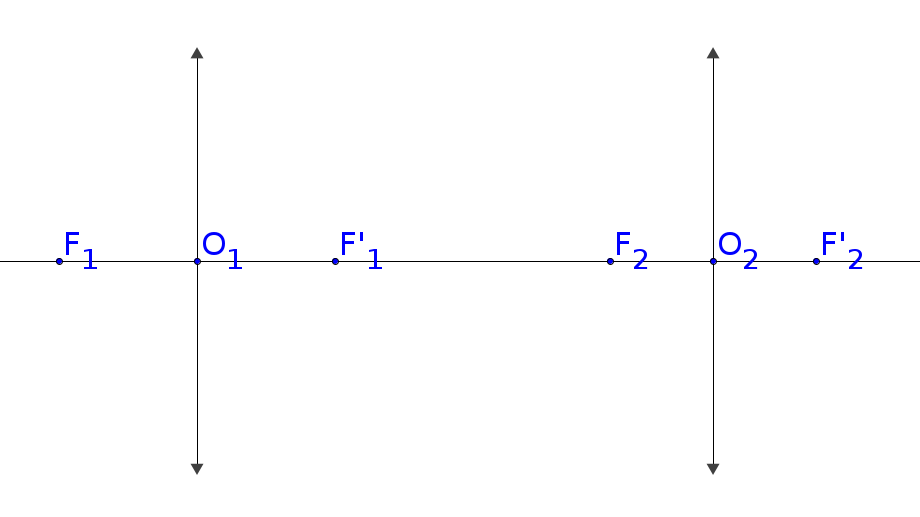
\includegraphics[width=\textwidth]{/home/chams/Documents/Travail/2024-2025/Colles/Images/mpsi_s05_ex02.png}
\end{minipage}%
\begin{minipage}[c]{\linewidth/2}
	On donne $\overline{O_1O_2} = D_0 = \SI{75}{mm}$, $f'_1 = \SI{10}{mm}$ et $f'_2 = \SI{25}{mm}$.
\end{minipage}
 
\begin{enumerate}
	\item Que sont les conditions de Gauss et à quoi servent elles ?
	\item On pose $\Delta = \overline{F'_1F'_2}$. Exprimer $\Delta$ en fonction des données du problème. Calcul.
	\item On souhaite qu'un œil au repos voie l'image $A'B'$ de $AB$ par le système optique. Où est $A'B'$.
	\item Où doit alors être l'image intermédiaire $A_1B_1$ ?
	\item Exprimer la position de l'objet $AB$ en fonction de $f'_1$ et $\Delta$. Calcul.
	\item Étude du grossissement :
	\begin{enumerate}
		\item Quelle est la taille maximale de l'image que l'on peut avoir sur la rétine sans microscope ?
		\item Quelle est la taille de l'image sur la rétine avec microscope ?
		\item En déduire le "grossissement commercial" du microscope.
	\end{enumerate}
\end{enumerate}

\subsection{Exercice 3 : Lunette astronomique}

On souhaite observer Mars. Soit $\alpha$ le diamètre angulaire sous lequel elle est vue à l'œil nu. Pour cela on utilise un système optique composé de deux lentilles convergentes de focales respectives $f'_1=f'_{obj}$ et $f'_2=f'_{oc}$ (l'oculaire est du côté de l'œil, l'objectif est du côté de l'objet Mars).

\begin{enumerate}
	\item On utilise un système afocal. Définir afocal. En déduire la position relative des deux lentilles.
	\item Faire le tracé des rayons. L'image est-elle droite ou renversée ?
	\item Soit $\alpha'$ le diamètre angulaire en sortie du système optique. Exprimer le grossissement $G = \alpha'/\alpha$. Interpréter cette grandeur.
	\item \label{qprec} On veut augmenter le grossissement et renverser l'image. On interpose entre l'objectif et l'oculaire une troisième lentille convergente de focale $f'_3$. On déplace l'oculaire pour pouvoir observer l'image au repos. Quel couple de points cette nouvelle lentille doit elle conjuguer ?
	\item Faire le tracé des rayons.
	\item Soit $\gamma_3$ le grandissement de la nouvelle lentille associé au couple de points de la question \ref{qprec}. Exprimer $\overline{O_3F'_{obj}}$ en fonction de $\gamma_3$ et $f'_3$.
	\item Quel est le grossissement $G'$ de ce nouveau système optique. Le comparer à $G$ et conclure.
\end{enumerate}
